\input{pre}

\tikzset{rrail/.style={rground,yscale=-1}}
\newcommand{\reffig}[1]{Fig.~\ref{#1}}

\begin{document}
\input{frontpage}
\newpage
\section{Simulating the Axon-Hillock Circuit}
\begin{figure}
    \center
    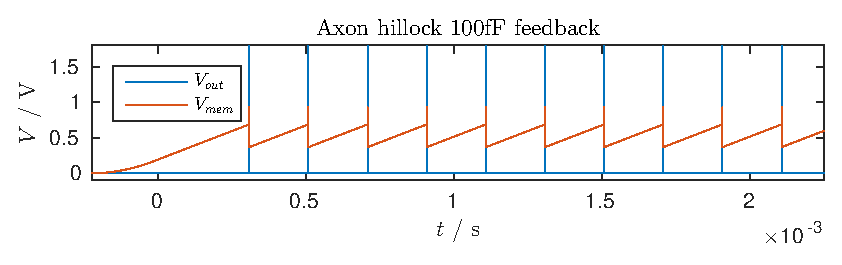
\includegraphics{fig1.eps}
    \caption{With \(V_{pw}=0.6\) and a 100fF feedback capacitor, our axon-hillock circuit produces 10 spikes in 2.25ms when
    fed with an input current of 1nA.}
    \label{fig:1}
\end{figure}
\begin{figure}
    \center
    \includegraphics{fig2.eps}
    \caption{Reducing the feedback capacitance to 50fF decreases the interspike interval.}
    \label{fig:2}
\end{figure}
\subsection{Simulation parameters}
\begin{itemize}
    \item iabstol: Determines the absolute tolerance for current calculation convergence. Default
        value \(1\cdot10^{-12}\).
    \item vabstol: Determines the absolute tolerance for voltage calculation convergence. Default
        value \(1\cdot10^{-6}\).
    \item gmin: The smallest conductance for non-linear components. Default value \(1\cdot10^{-12}\).
    \item reltol: Relative tolerance for convergence between two time steps. Default value \(1\cdot10^{-4}\).
\end{itemize}
When doing a transient analysis, the simulator determines the size of the time steps such that the difference
in voltage between two timesteps \(t_{k}\) and \(t_{k+1}\) is smaller than
\begin{equation*}
    |V(t_{k+1}) - V(t_{k})| < |V(t_{k+1}) - V(t_{k})|\cdot \text{reltol} + \text{vabstol}
\end{equation*}
And for the current difference between two time steps
\begin{equation*}
    |I(t_{k+1}) - I(t_{k})| < |I(t_{k+1}) - I(t_{k})|\cdot \text{reltol} + \text{iabstol}
\end{equation*}
Making the tolerances smaller increases the accuracy of the simulation at the expense of computational power.

\subsection{DC analysis}
DC analysis of the neuron circuit is problematic because the circuit does not have a fixed DC operating point. If
a DC current is injected into the circuit, the output will spike periodically instead of settling to a constant operating
point. Instead, we must perform a transient analysis.

\subsection{Transient analysis}
Fig.~\ref{fig:1} shows the result of doing a transient analysis of the axon hillock circuit, with the \texttt{sigrampup} option enabled.
\texttt{sigrampup} initiates the circuit with all sources at \(0\), at time \(t=-0.1T\) where T is the total simulation time. The sources
are then ramped up so that they reach their final value at time \(t=0\). 

We use \(\texttt{gmin} = 1\cdot10^{-15}\) and \(\texttt{iabstol} = 1\cdot10^{-15}\) for all simulations in this report. It is important
to use such small values for these parameters when dealing with the neuron circuits because they work with very small currents that need
to be accurately integrated over time to produce a correct simulation of the actual circuit dynamics.

\subsection{Feedback capacitor effect}
\begin{figure}
    \center
    \includegraphics{fig3.eps}
    \caption{A feedback capacitance of 250fF increases the interspike interval and causes larger swings in the membrane voltage.}
    \label{fig:3}
\end{figure}
\begin{figure}
    \center
    \includegraphics{fig4.eps}
    \caption{A feedback capacitance of 500fF gives a membrane to feedback capacitance ratio of 1. Spikes now couple back to the membrane
    potential so strongly that the membrane voltage becomes negative.}
    \label{fig:4}
\end{figure}
Figs.~\ref{fig:1} through~\ref{fig:4} show the axon hillock response for feedback capacitance values of 100fF, 50fF, 250fF and 500fF in that order.
Since the change in membrane potential from a spike is given by
\begin{equation*}
    \Delta V_{mem} = \frac{C_{f}}{C_f+C_{mem}} V_{dd}
\end{equation*}
larger feedback capacitances cause a greater swing in membrane potential, even causing it to become negative when using the 500fF feedback capacitor.
The time between spikes also increases with increasing feedback capacitance because the charging time is given by
\begin{equation*}
    T_L = \frac{(C_f+C_{mem})\Delta V_{mem}}{I_{in}} = \frac{C_fV_{dd}}{I_{in}}
\end{equation*}
The time spent on the spike is given by
\begin{equation*}
    T_H = \frac{(C_f+C_{mem})\Delta V_{mem}}{I_r-I_{in}} = \frac{C_fV_{dd}}{I_r-I_{in}}
\end{equation*}
And does not change by a noticeable amount, indicating that the draining current is very large compared to the charging current.
This is clearly shown in Fig.~\ref{fig:zoomed} which depicts a close-up of two spikes from Fig.~\ref{fig:1}.
\begin{figure}
    \center
    \includegraphics{fig_zoom.eps}
    \caption{A zoomed version of the spike train in Fig.~\ref{fig:1}. The discharge time of the membrane capacitor is clearly negligible compared to the charge time.}
    \label{fig:zoomed}
\end{figure}
\begin{figure}
    \center
    \includegraphics{fig5.eps}
    \caption{Changed \(V_{pw}\) to \(0.2\) decreases the maximum discharge current and therefore increases the time that the membrance capacitor spends discharging.}
    \label{fig:5}
\end{figure}
\subsection{Axon-Hillock power consumption}
We measured the average current through the first inverter to be \(5.327\mu\)A, and the current through the circuit's power supply to be \(5.365\mu\)A. The circuit
is supplied with 1.8 volts and therefore the power consumption is
\begin{equation*}
    P_{inv} = 9.589 \mu\text{W}, \quad  P_{tot} = 9.657 \mu\text{W}
\end{equation*}
The first inverter therefore consumes 99.3\% of the total power consumed by the circuit, ignoring the power provided by the input current source.
\begin{figure}
    \center
    \includegraphics{fig6.eps}
    \caption{The low power soma shows a different membrane charging characteristic from the axon-hillock circuit. Here we generate 10 spikes in 2.25ms 
    using an input current of 275pA and a refractory period set by $V_r=0.25$V.}
    \label{fig:6}
\end{figure}
\section{Low Power Neuron Circuit}
Fig.~\ref{fig:6} shows the response of the low power neuron circuit when injected with an input current of 275pA. The average current going through the
first inverter for the simulation shown in Fig.~\ref{fig:6} was 1.396nA, and the current through the power supply was 2.55nA. The power consumed by the
inverter and in total is therefore
\begin{equation*}
    P_{inv} = 2.513 \text{nW}, \quad  P_{tot} = 4.59 \text{nW}
\end{equation*}
The first inverter therefore consumes 55.7\% of the total power in the low power neuron circuit.

Compared to the axon-hillock circuit, the low power neuron consumes about 2100 times less power.
The reason for this is the positive feedback from the first inverter in the low power neuron. This feedback speeds up the response of the first inverter, which 
then spends less time in the I-V relationship region where it consumes significant amounts of power.

\newpage
\appendix
\section{Appendix: Schematics of Created Circuits}
\begin{figure}[!h]
    \includegraphics[width=\textwidth]{axhil.png}
    \caption{Axon-Hillock circuit.}
\end{figure}
\begin{figure}[!h]
    \includegraphics[width=\textwidth]{soma_lowpower.png}
    \caption{Low power neuron circuit.}
\end{figure}
\end{document}
